\section{Exercises}
\subsection{Estimating unknown parameters}

%\Comment{added 1-4 from OpenIntro Stat chapter 4 foundations for inference, though 3 and 4 deal with means rather than proportions.  seems like students should still be able to answer these questions (i added a hint to the last part), but might want to rewrite later.  The rest of the questions are from ISRS foundations of inference.}
%\Comment{need to add in more conceptual questions about ci and tests.  Need to add in questions about type 1 and type 2 errors and power}

% 1

\eoce{\qt{Identify the parameter, Part I} For each of the following situations, state whether the parameter of interest is a mean or a proportion. It may be helpful to examine whether individual responses are numerical or categorical.
\begin{parts}
\item In a survey, one hundred college students are asked how many hours per week they spend on the Internet.
\item In a survey, one hundred college students are asked: ``What percentage of the time you spend on the Internet is part of your course work?"
\item In a survey, one hundred college students are asked whether or not they cited information from Wikipedia in their papers.
\item In a survey, one hundred college students are asked what percentage of their total weekly spending is on alcoholic beverages.
\item In a sample of one hundred recent college graduates, it is found that 85 percent expect to get a job within one year of their graduation date.
\end{parts}
}{}

% 2

\eoce{\qt{Identify the parameter, Part II} For each of the following situations, state whether the parameter of interest is a mean or a proportion. 
\begin{parts}
\item A poll shows that 64\% of Americans personally worry a great deal about federal spending and the budget deficit.
\item A survey reports that local TV news has shown a 17\% increase in revenue between 2009 and 2011 while newspaper revenues decreased by 6.4\% during this time period.
\item In a survey, high school and college students are asked whether or not they use geolocation services on their smart phones.
\item In a survey, internet users are asked whether or not they purchased any Groupon coupons.
\item In a survey, internet users are asked how many Groupon coupons they purchased over the last year.
\end{parts}
}{}

% 3
\textPE{\newpage}

\eoce{\qt{College credits} \label{credits} A college counselor is interested in estimating how many credits a student typically enrolls in each semester. The counselor decides to randomly sample 100 students by using the registrar's database of students. The histogram below shows the distribution of the number of credits taken by these students. Sample statistics for this distribution are also provided.\\
\begin{minipage}[c]{0.7\textwidth}
\begin{center}
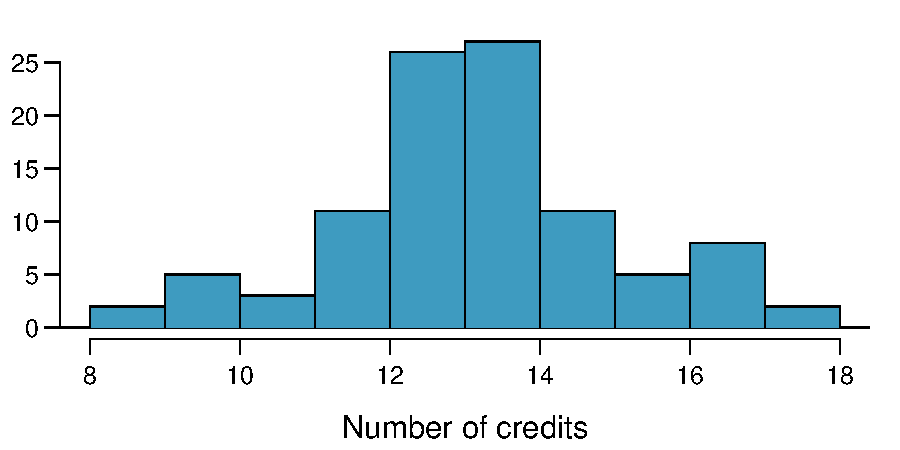
\includegraphics[width=96mm]{ch_distributions/figures/eoce/credits/credits}
\end{center}
\end{minipage}
\begin{minipage}[c]{0.3\textwidth}
\begin{center}
\begin{tabular}{l|r l}
Min		& 8 \\
Q1		& 13 \\
Median	& 14 \\
Mean	& 13.65 \\
SD		& 1.91 \\
Q3		& 15 \\
Max		& 18 \\
\end{tabular}
\end{center}
\end{minipage}
\begin{parts}
\item What is the point estimate for the average number of credits taken per semester by students at this college? What about the median?
\item What is the point estimate for the standard deviation of the number of credits taken per semester by students at this college? What about the IQR?
\item Is a load of 16 credits unusually high for this college? What about 18 credits? Explain your reasoning. \textit{Hint:} Observations farther than two standard deviations from the mean are usually considered to be unusual.
\item The college counselor takes another random sample of 100 students and this time finds a sample mean of 14.02 units. Should she be surprised that this sample statistic is slightly different than the one from the original sample? Explain your reasoning.
\item The sample means given above are point estimates for the mean number of credits taken by all students at that college. What measures do we use to quantify the variability of this estimate (Hint: recall that $SD_{\bar{x}}=\frac{\sigma}{\sqrt{n}}$)? Compute this quantity using the data from the original sample.\end{parts}
}{}

% 4

\eoce{\qt{Heights of adults} \label{heights} Researchers studying anthropometry collected body girth measurements and skeletal diameter measurements, as well as age, weight, height and gender, for 507 physically active individuals. The histogram below shows the sample distribution of heights in centimeters. \footfullcite{Heinz:2003} \\
\begin{minipage}[c]{0.7\textwidth}
\begin{center}
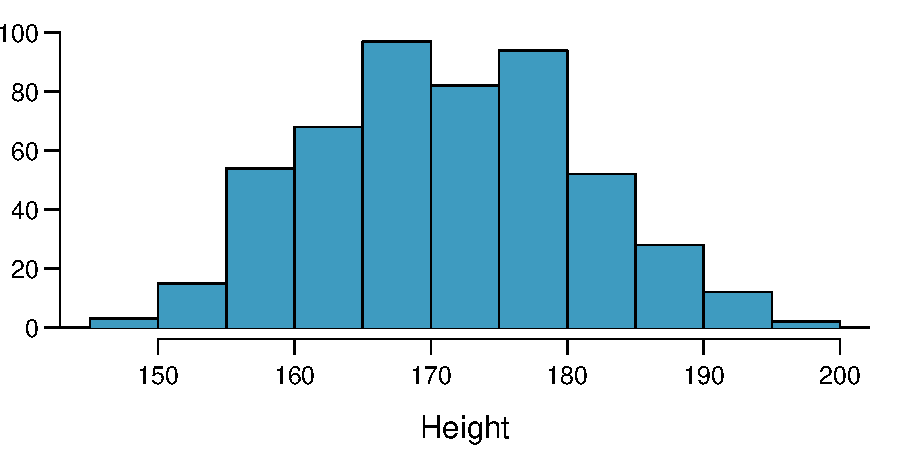
\includegraphics[width=85mm]{ch_distributions/figures/eoce/bdims/bdims_heights}
\end{center}
\end{minipage}
\begin{minipage}[c]{0.3\textwidth}
\begin{center}
\begin{tabular}{l|r l}
Min		& 147.2 \\
Q1		& 163.8 \\
Median	& 170.3 \\
Mean	& 171.1 \\
SD		&  9.4 \\
Q3		& 177.8 \\
Max		& 198.1 \\
\end{tabular}
\end{center}
\end{minipage}
\begin{parts}
\item What is the point estimate for the average height of active individuals? What about the median?
\item What is the point estimate for the standard deviation of the heights of active individuals? What about the IQR? \textPE{\textbf{See the next page for parts (c)-(e).}\pagebreak}
\item Is a person who is 1m 80cm (180 cm) tall considered unusually tall? And is a person who is 1m 55cm (155cm) considered unusually short? Explain your reasoning.
\item The researchers take another random sample of physically active individuals. Would you expect the mean and the standard deviation of this new sample to be the ones given above? Explain your reasoning.
\item The sample means obtained are point estimates for the mean height of all active individuals, if the sample of individuals is equivalent to a simple random sample. What measure do we use to quantify the variability of such an estimate (Hint: recall that $SD_{\bar{x}}=\frac{\sigma}{\sqrt{n}}$)? Compute this quantity using the data from the original sample under the condition that the data are a simple random sample. 
\end{parts}
}{}

%\textPE{\newpage}


%_________________
\subsection{Confidence intervals} % (Section~\ref{})}
% 5

\eoce{\qt{Chronic illness, Part I} \label{ChronicIllnessP1}
In 2013, the Pew Research Foundation reported that ``45\% of U.S. adults report that they live with one or more chronic conditions''.\footnote{\href{http://pewinternet.org/Reports/2013/The-Diagnosis-Difference.aspx}{The Diagnosis Difference}. November 26, 2013. Pew Research.} However, this value was based on a sample, so it may not be a perfect estimate for the population parameter of interest on its own. The study reported a standard error of about 1.2\%, and a normal model may reasonably be used in this setting. Create a 95\% confidence interval for the proportion of U.S. adults who live with one or more chronic conditions. Also interpret the confidence interval in the context of the study.}
{
%$0.45 \pm 1.96 \times 0.012 = (0.426, 0.474)$ \\
%We are 95\% confident that 42.6\% to 47.4\% of U.S. adults live with one or more chronic conditions.
}

% 6

\eoce{\qt{Twitter users and news, Part I} A poll conducted in 2013 found that 52\% of U.S. adult Twitter users get at least some news on Twitter.\footnote{\href{http://www.journalism.org/2013/11/04/twitter-news-consumers-young-mobile-and-educated}{Twitter News Consumers: Young, Mobile and Educated}. November 4, 2013. Pew Research.} The standard error for this estimate was 2.4\%, and a normal distribution may be used to model the sample proportion. Construct a 99\% confidence interval for the fraction of U.S. adult Twitter users who get some news on Twitter, and interpret the confidence interval in context.}{}

%%%\textA{\pagebreak}

% 7

\eoce{\qt{Chronic illness, Part II} In 2013, the Pew Research Foundation reported that ``45\% of U.S. adults report that they live with one or more chronic conditions'', and the standard error for this estimate is 1.2\%.
Identify each of the following statements as true or false. Provide an explanation to justify each of your answers.
\begin{parts}
\item We can say with certainty that the confidence interval from Exerise~\ref{ChronicIllnessP1} contains the true percentage of U.S. adults who suffer from a chronic illness.
\item If we repeated this study 1,000 times and constructed a 95\% confidence interval for each study, then approximately 950 of those confidence intervals would contain the true fraction of U.S. adults who suffer from chronic illnesses.
\item The poll provides statistically significant evidence (at the $\alpha = 0.05$ level) that the percentage of U.S. adults who suffer from chronic illnesses is below 50\%.
\item Since the standard error is 1.2\%, only 1.2\% of people in the study communicated uncertainty about their answer.
\end{parts}}
{
%\begin{parts}
%\item False, we're only 95\% confident.
%\item True, this is the definition of the confidence level.
%\item True, the equivalent significance level of a one sided hypothesis test for a 95\% confidence interval is indeed 2.5\%, and since the interval lies below 50\% this statement is correct. % would need revision of this part
%\item False, the 1.2\% measures the uncertainty associated with the sample proportion (the point estimate) not the uncertainty of individual observations, uncertainty in the sense of not being sure of one's answer to a survey question.
%\end{parts}
}

% 8
\textPE{\pagebreak}

\eoce{\qt{Twitter users and news, Part II} A poll conducted in 2013 found that 52\% of U.S. adult Twitter users get at least some news on Twitter, and the standard error for this estimate was 2.4\%. Identify each of the following statements as true or false. Provide an explanation to justify each of your answers.
\begin{parts}
\item The data provide statistically significant evidence that more than half of U.S. adult Twitter users get some news through Twitter. Use a significance level of $\alpha = 0.01$.
\item Since the standard error is 2.4\%, we can conclude that 97.6\% of all U.S. adult Twitter users were included in the study.
\item If we want to reduce the standard error of the estimate, we should collect less data.
\item If we construct a 90\% confidence interval for the percentage of U.S. adults Twitter users who get some news through Twitter, this confidence interval will be wider than a corresponding 99\% confidence interval.
\end{parts}}{}


%_________________
\subsection{Introducing hypothesis tests}

% 9

\eoce{\qt{Social experiment, Part I} \label{socExpP1} A ``social experiment" conducted by a TV program questioned what people do when they see a very obviously bruised woman getting picked on by her boyfriend. On two different occasions at the same restaurant, the same couple was depicted. In one scenario the woman was dressed ``provocatively'' and in the other scenario the woman was dressed ``conservatively''. The table below shows how many restaurant diners were present under each scenario, and whether or not they intervened.
\begin{center}
\begin{tabular}{ll cc c} 
			&				& \multicolumn{2}{c}{\textit{Scenario}} \\
\cline{3-4}
							&			& Provocative	& Conservative 	& Total	\\
\cline{2-5}
\multirow{2}{*}{\textit{Intervene}}	&Yes 		& 5	 	& 15		& 20 	\\
							&No			& 15	 	& 10 	 	& 25 \\
\cline{2-5}
							&Total		& 20		& 25		& 45 \\
\end{tabular}
\end{center}
A simulation was conducted to test if people react differently under the two scenarios. 10,000 simulated differences were generated to construct the null distribution shown. The value $\hat{p}_{pr, sim}$ represents the proportion of diners who intervened in the simulation for the provocatively dressed woman, and $\hat{p}_{con, sim}$ is the proportion for the conservatively dressed woman.
\begin{center}
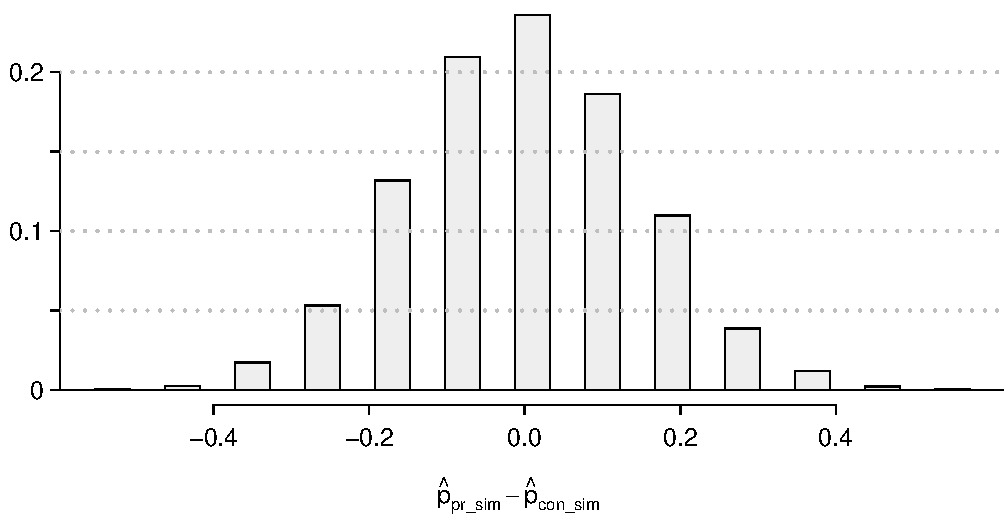
\includegraphics[width=0.7\textwidth]{ch_inference_for_props/figures/eoce/socExp/socExp}
\end{center}
\begin{parts}
\item What are the hypotheses? For the purposes of this exercise, you may assume that each observed person at the restaurant behaved independently, though we would want to evaluate this assumption more rigorously if we were reporting these results.
\item Calculate the observed difference between the rates of intervention under the provocative and conservative scenarios: $\hat{p}_{pr} - \hat{p}_{con}$.
\item Estimate the p-value using the figure above and determine the conclusion of the hypothesis test.
\end{parts}
}{}

%%%\textA{\newpage}


% 10

\eoce{\qt{Is yawning contagious, Part I} \label{yawningContageousP1} An experiment conducted by the \textit{MythBusters}, a science entertainment TV program on the Discovery Channel, tested if a person can be subconsciously influenced into yawning if another person near them yawns. 50 people were randomly assigned to two groups: 34 to a group where a person near them yawned (treatment) and 16 to a group where there wasn't a person yawning near them (control). The following table shows the results of this experiment. \footfullcite{data:yawn}
\begin{center}
\begin{tabular}{ll cc c} 
			&				& \multicolumn{2}{c}{\textit{Group}} \\
\cline{3-4}
							&			& Treatment	& Control 	& Total	\\
\cline{2-5}
\multirow{2}{*}{\textit{Result}}		&Yawn 		& 10	 	& 4		& 14 	\\
							&Not Yawn	& 24	 	& 12 	 	& 36 \\
\cline{2-5}
							&Total		& 34		& 16		& 50 \\
\end{tabular}
\end{center}
A simulation was conducted to understand the distribution of the test statistic under the assumption of independence: having someone yawn near another person has no influence on if the other person will yawn. In order to conduct the simulation, a researcher wrote yawn on 14 index cards and not yawn on 36 index cards to indicate whether or not a person yawned. Then he shuffled the cards and dealt them into two groups of size 34 and 16 for treatment and control, respectively. He counted how many participants in each simulated group yawned in an apparent response to a nearby yawning person, and calculated the difference between the simulated proportions of yawning as $\hat{p}_{trtmt,sim} - \hat{p}_{ctrl,sim}$. This simulation was repeated 10,000 times using software to obtain 10,000 differences that are due to chance alone. The histogram shows the distribution of the simulated differences.
\begin{center}
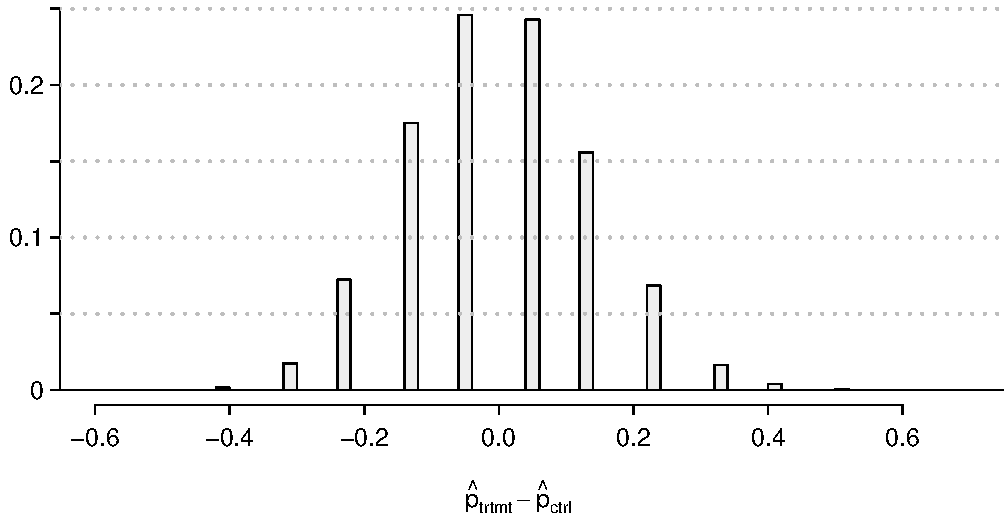
\includegraphics[width=0.9\textwidth]{ch_inference_for_props/figures/eoce/yawn/yawn}
\end{center}

\begin{parts}
\item What are the hypotheses?
\item Calculate the observed difference between the yawning rates under the two scenarios.
\item Estimate the p-value using the figure above and determine the conclusion of the hypothesis test.
\end{parts}
}{}

%%%\textA{\pagebreak}

% 11

\eoce{\qt{Social experiment, Part II} In Exercise~\ref{socExpP1}, we encountered a scenario where researchers were evaluating the impact of the way someone is dressed against the actions of people around them. In that exercise, researchers may have believed that dressing provocatively may reduce the chance of bystander intervention. One might be tempted to use a one-sided hypothesis test for this study. Discuss the drawbacks of doing so in 1-3 sentences.}{}

% 12

\eoce{\qt{Is yawning contagious, Part II} Exercise~\ref{yawningContageousP1} describes an experiment by Myth Busters, where they examined whether a person yawning would affect whether others to yawn. The traditional belief is that yawning is contagious -- one yawn can lead to another yawn, which might lead to another, and so on. In that exercise, there was the option of selecting a one-sided or two-sided test. Which would you recommend (or which did you choose)? Justify your answer in 1-3 sentences.}{}




% 13

\eoce{\qt{The Egyptian Revolution} \label{EgyptianRevolutionEOCE} A popular uprising that started on January 25, 2011 in Egypt led to the 2011 Egyptian Revolution. Polls show that about 69\% of American adults followed the news about the political crisis and demonstrations in Egypt closely during the first couple weeks following the start of the uprising. Among a random sample of 30 high school students, it was found that only 17 of them followed the news about Egypt closely during this time. \footfullcite{data:egypt}

\begin{parts}

\item Write the hypotheses for testing if the proportion of high school students who followed the news about Egypt is different than the proportion of American adults who did.

\item Calculate the proportion of high schoolers in this sample who followed the news about Egypt closely during this time.

\item Describe how to perform a simulation and, once you had results, how to estimate the p-value.

\item Below is a histogram showing the distribution of $\hat{p}_{sim}$ in 10,000 simulations under the null hypothesis. Estimate the p-value using the plot and determine the conclusion of the hypothesis test.
\begin{center}
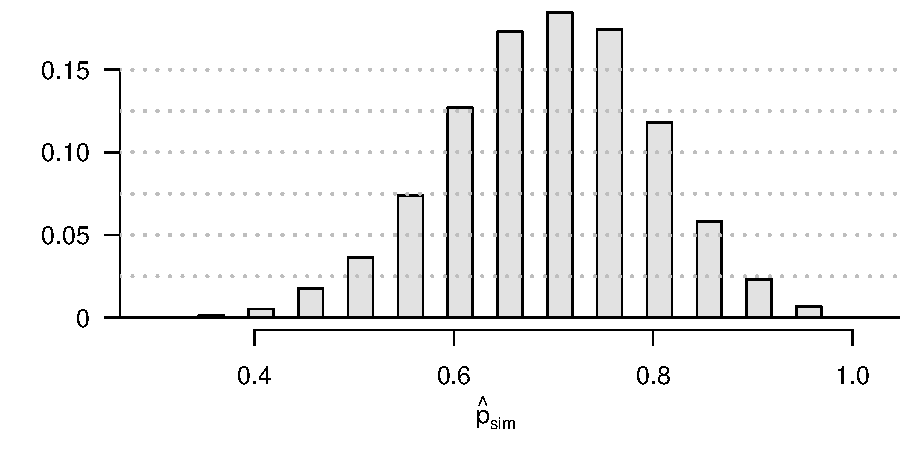
\includegraphics[width=0.65\textwidth]{ch_inference_for_props/figures/eoce/egypt/egypt}
\end{center}

\end{parts}
}{}

% 14
\textPE{\newpage}

\eoce{\qt{Assisted Reproduction} \label{AssistedReproductionEOCE} Assisted Reproductive Technology (ART) is a collection of techniques that help facilitate pregnancy (e.g. in vitro fertilization). A 2008 report by the Centers for Disease Control and Prevention estimated that ART has been successful in leading to a live birth in 31\% of cases \footfullcite{web:art}. A new fertility clinic claims that their success rate is higher than average. A random sample of 30 of their patients yielded a success rate of 40\%. A consumer watchdog group would like to determine if this provides strong evidence to support the company's claim.
\begin{parts}
\item Write the hypotheses to test if the success rate for ART at this clinic is significantly higher than the success rate reported by the CDC.
\item Describe a setup for a simulation that would be appropriate in this situation and how the p-value can be calculated using the simulation results.
\item Below is a histogram showing the distribution of $\hat{p}_{sim}$ in 10,000 simulations under the null hypothesis. Estimate the p-value using the plot and use it to evaluate the hypotheses.
\item After performing this analysis, the consumer group releases the following news headline: ``Infertility clinic falsely advertises better success rates". Comment on the appropriateness of this statement.
\begin{center}
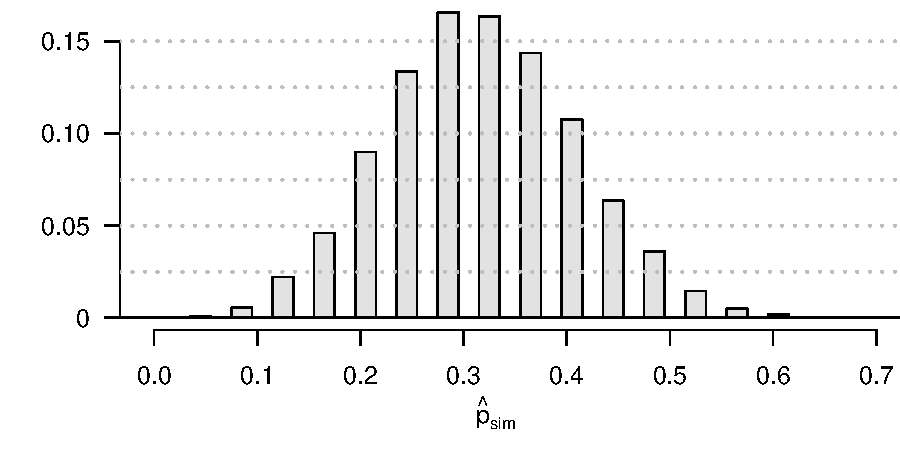
\includegraphics[width=0.7\textwidth]{ch_inference_for_props/figures/eoce/art/art}
\end{center}
\end{parts}
}{}




